Le système global est composé de quatre entités distinctes, décrites dans les sous-sections suivantes.

%%%%%%%%%%%%%%%%%%%%%%%%%%%%%%%%%%%%%%%%%%%%%%%%%%%%%%%%%%%%%%%%%%%%%%%%%%%%%%%%%%%%%%%%%%%%%%%%%%%
%%%%%%%%%%%%%%%%%%%%%%%%%%%%%%%%%%%%%%%%%%%%%%%%%%%%%%%%%%%%%%%%%%%%%%%%%%%%%%%%%%%%%%%%%%%%%%%%%%%
\subsection{Gestion des tags}
La gestion physiques des tags stockés dans les attributs étendus (\acrshort{xattr}) est une fonctionnalité indépendante du 
reste du système. Comme vu dans la section \ref{extended_attributes}, des outils système existent pour 
manipuler les \acrshort{xattr} des fichiers. Cependant, pour offrir un plus haut niveau d'abstraction, 
une cohérence sur le nommage des tags pour l'indexation et plus de confort pour l'utilisateur final, 
un outil devient nécessaire pour la gestion des tags. Cet outil se présente, sous sa forme de base, 
comme un programme en ligne de commande. Il doit, au minimum, offrir la possibilité de lire les tags 
contenus dans les fichiers et ajouter et supprimer les tags donnés en entrée par l'utilisateur. 
Il devra pouvoir manipuler plusieurs tags et fichiers simultanément. D'un point de vue algorithmique 
et structures de données, cette partie n'est pas particulièrement ardue.

%%%%%%%%%%%%%%%%%%%%%%%%%%%%%%%%%%%%%%%%%%%%%%%%%%%%%%%%%%%%%%%%%%%%%%%%%%%%%%%%%%%%%%%%%%%%%%%%%%%
%%%%%%%%%%%%%%%%%%%%%%%%%%%%%%%%%%%%%%%%%%%%%%%%%%%%%%%%%%%%%%%%%%%%%%%%%%%%%%%%%%%%%%%%%%%%%%%%%%%
\subsection{Indexation des fichiers et des tags}
L'indexation des fichiers et des tags associés est l'un des deux piliers du système. Il faut créer 
un index des relations entre les tags et les fichiers. Le terme "index" utilisé ici ne 
prend pas son sens littéraire exact, \textit{id est} la liste des termes importants 
d'un livre avec la liste des pages dans lesquels ils apparaissent. Dans notre situation, il se 
rapproche plus de son utilisation pour les bases de données : c'est une structure de données 
permettant de retrouver rapidement les données, dans notre cas, récupérer rapidement la relation 
entre tags et fichiers. Deux architectures ont été imaginées pour l'indexation des tags et des fichiers, 
elles sont décrites dans les deux sous-sections suivantes. La table \ref{table_evenements_possibles} liste 
les événements qui se produisent lors d'une utilisation normale du \acrshort{fs} en leur attribuant 
un numéro. Ces numéros sont repris et utilisés pour alléger la lecture des tables \ref{table_architecture_1} 
et \ref{table_architecture_2}.
\begin{center}
    \begin{tabularx}{15cm}{|c|X|} \hline
        \textbf{Numéro} & \textbf{Cas d'utilisation} \\ \hline
        1 & Ajout d'un tag à un fichier ou à un répertoire \\ \hline
        2 & Suppression d'un tag d'un fichier ou à un répertoire \\ \hline
        3 & Renommage d'un tag \\ \hline
        4 & Ajout d'un fichier dans l'arborescence surveillée \\ \hline
        5 & Ajout d'un répertoire dans l'arborescence surveillée \\ \hline
        6 & Déplacement ou renommage d'un fichier dans l'arborescence surveillée \\ \hline
        7 & Déplacement ou renommage d'un répertoire dans l'arborescence surveillée \\ \hline
        8 & Suppression d'un fichier de l'arborescence surveillée \\ \hline
        9 & Suppression d'un répertoire de l'arborescence surveillée \\ \hline
    \end{tabularx}
    \captionof{table}{Événements survenant sur le \acrshort{fs}}
    \label{table_evenements_possibles}
\end{center}
Les explications suivantes mentionnent la notion de \textbf{complexité en temps} (le nombre d'opérations 
nécessaires à l'accomplissement de l'algorithme, en fonction de la taille des entrées) avec la notation 
de Landau, ou \textit{Big O} \cite{ref54}.

%%%%%%%%%%%%%%%%%%%%%%%%%%%%%%%%%%%%%%%%%%%%%%%%%%%%%%%%%%%%%%%%%%%%%%%%%%%%%%%%%%%%%%%%%%%%%%%%%%%
%%%%%%%%%%%%%%%%%%%%%%%%%%%%%%%%%%%%%%%%%%%%%%%%%%%%%%%%%%%%%%%%%%%%%%%%%%%%%%%%%%%%%%%%%%%%%%%%%%%
\subsubsection{Indexation avec table de hachage et arbre}\label{indexation_hashmap_arbre}
La première version de l'architecture de l'indexation, comportant deux structures de données, est la suivante :
\begin{enumerate}
    \item Une table de hachage (ou \textit{hashmap}) associant un tag (son nom, sous forme de 
        chaîne de caractères) à un ensemble (au sens mathématique) de chemins de fichiers sur 
        le disque.
    \item Un arbre, correspondant à l'arborescence des fichiers, avec comme noeuds les répertoires, 
        sous-répertoires et fichiers. Le répertoire à surveiller représente la racine de l'arbre.
        Les liens entre les noeuds représentent le contenu d'un répertoire. Les données du noeud 
        contiennent le nom du fichier ou du répertoire et l'ensemble des tags associés au fichier.
\end{enumerate}
\begin{figure}
    \begin{center}
        \fbox{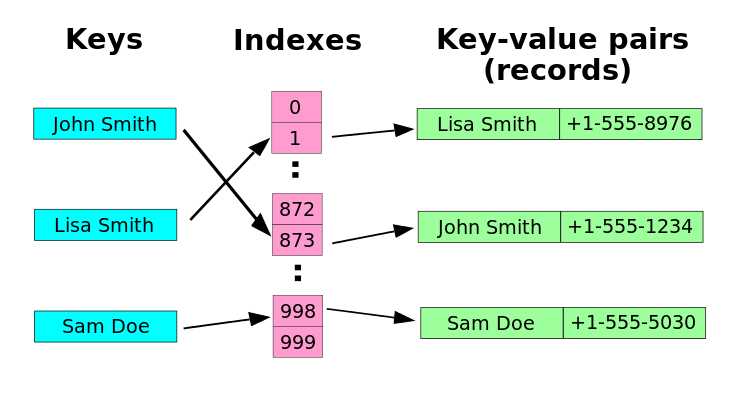
\includegraphics[width=0.7\textwidth]{images/hashmap_wiki.png}}
    \end{center}
    \caption{Un annuaire représenté comme une table de hachage - \cite{ref27}}
    \label{hashmap_wiki}
\end{figure}
Une table de hachage est un tableau associatif. Les composantes de l'association sont la "clé", 
reliée à une ou plusieurs valeurs. Pour insérer, accéder ou supprimer une entrée de la table, 
il faut calculer le "hash" de la clé, \textit{id est} son empreinte unique. Sur la figure \ref{hashmap_wiki}, 
nous apercevons les clés en bleu, le résultat du hash en rouge et les valeurs associées en vert. 
Le risque que deux clés ou plus produisent une même empreinte s'appelle une "collision", c'est 
pour cela qu'une bonne implémentation d'une table de hachage doit non seulement utiliser une bonne 
fonction de hachage mais aussi une manière de résoudre les collisions. C'est ainsi que les trois 
opérations ci-dessus peuvent être réalisées, en moyenne, en temps constant (O(1)) et dans le pire 
des cas (si les collisions s'enchainent) en temps linéaire (O(n)). Dans notre cas, l'utilisation 
d'une table de hachage pour stocker la relation entre un tag et ses fichiers est efficace lorsqu'une 
recherche par tags est demandée. De plus, en associant un ensemble de chemins de fichiers, 
des opérations ensemblistes (union, intersection) peuvent être réalisées lorsque une recherche 
impliquant plusieurs tags est effectuée.
\bigbreak
L'arbre, au sens informatique, est une représentation de la hiérarchie du \acrshort{fs} dans 
notre cas. Prenons comme exemple la hiérarchie suivante :
\dirtree{%
.1 home.
.2 root.
.2 user.
.3 docs.
.4 graph.pdf.
.4 report.tex.
.3 images.
.4 img1.png.
.4 img2.png.
.3 music.
.4 kiss.mp3.
}
Elle peut être obtenue grâce à la commande \mintinline{bash}{tree} sous Linux par exemple.
La même représentation sous forme d'un arbre est illustrée sur la figure \ref{tree} :
\begin{figure}
    \begin{center}
        \fbox{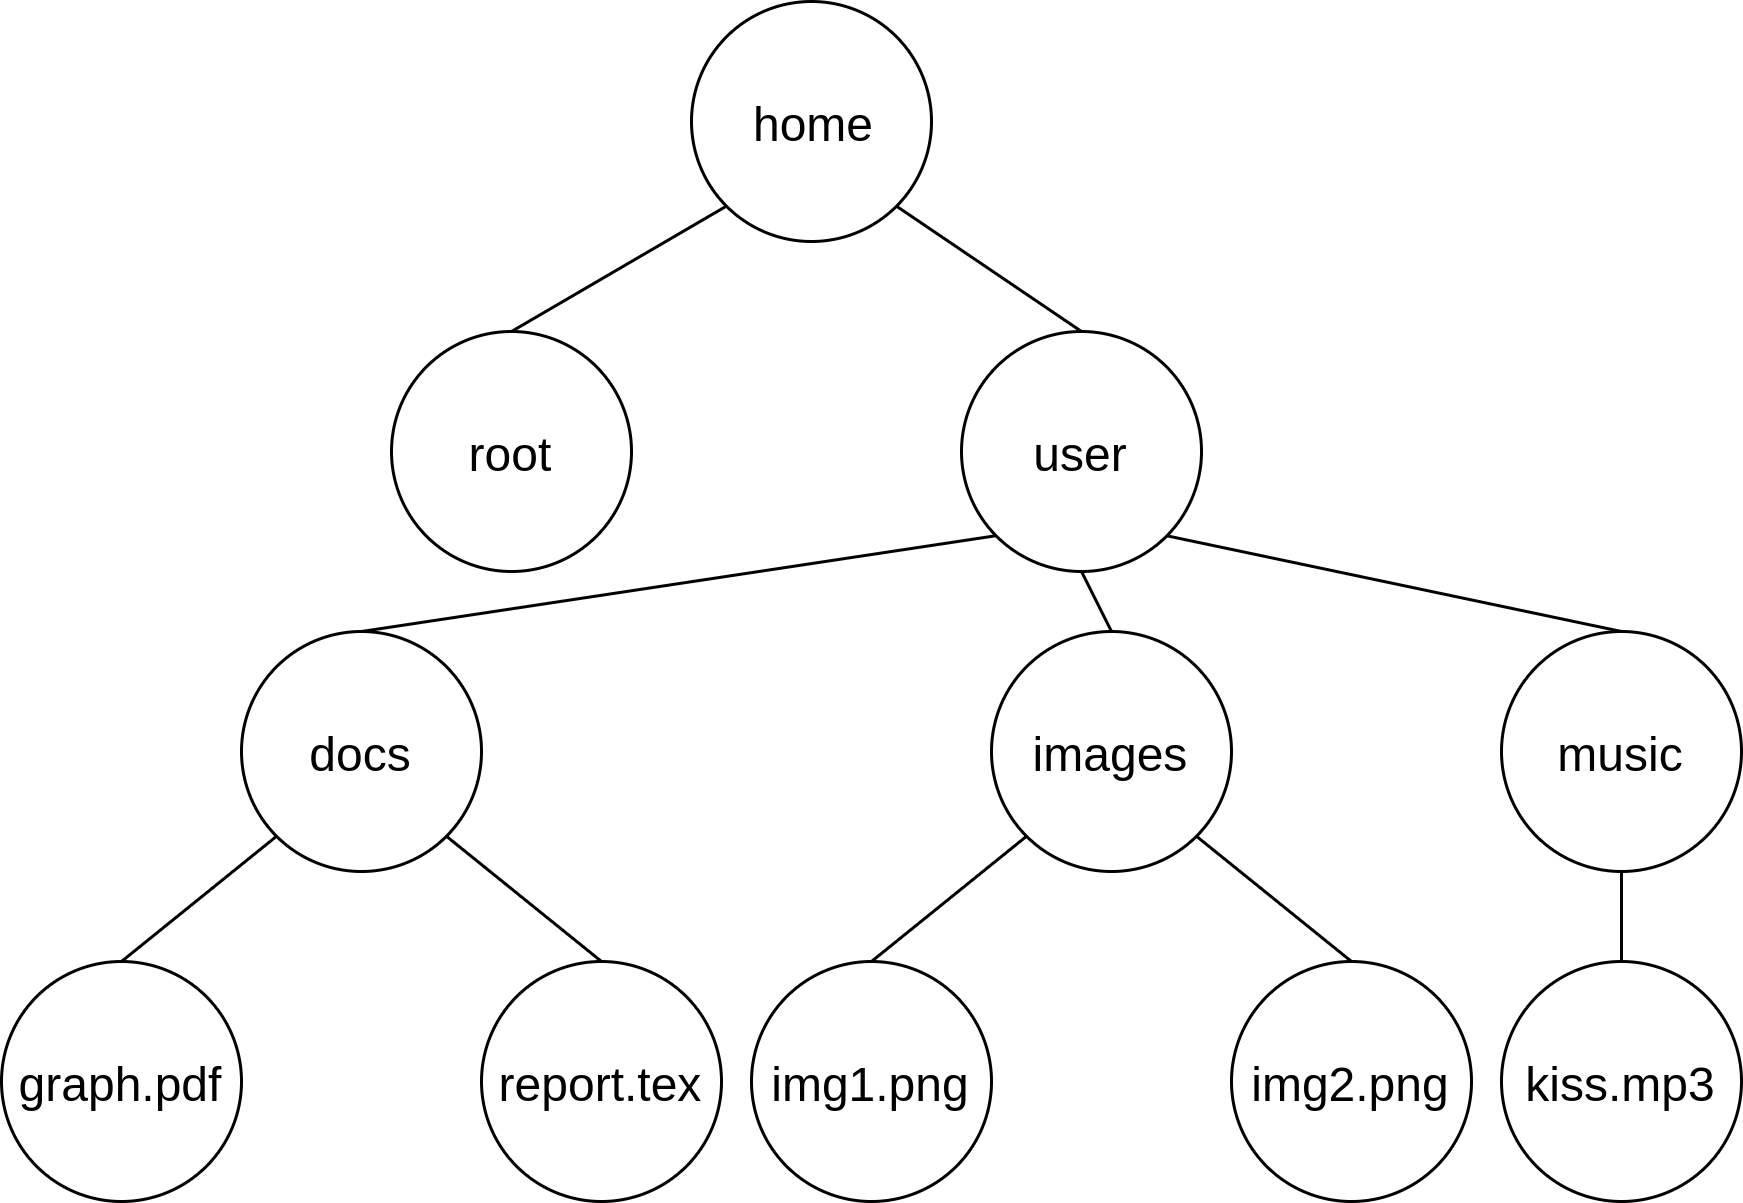
\includegraphics[width=0.8\textwidth]{images/tree.png}}
    \end{center}
    \caption{Représentation sous forme d'arbre d'une hiérarchie de fichiers et répertoires}
    \label{tree}
\end{figure}
Le noeud "home" représente la racine de l'arbre. Chaque noeud représente soit un fichier (en orange), soit 
un répertoire (en bleu) sur le disque. Chaque répertoire peut être vu comme un sous-arbre de l'arbre principal.
Du point de vue programmatoire, un noeud serait défini, au minimum, comme une structure de données 
contenant un champ "données" (dans notre cas, le nom du fichier/répertoire et l'ensemble de ses tags) 
et un champ "enfants", une liste ou un ensemble de pointeurs vers les noeuds enfants. Dans le cas 
présent, seuls les noeuds répertoires pointent vers des noeuds répertoires ou fichiers enfants, 
les fichiers n'auraient qu'une liste vide de pointeurs.
\bigbreak
La table \ref{table_architecture_1} donne, pour chaque événement survenu sur le \acrshort{fs}, les opérations 
à exécuter pour les deux structures de données (la table de hachage et l'arbre) et une approximation 
de la complexité. Les événements sont représentés par leurs numéros, en table 
\ref{table_evenements_possibles}. Les variables suivantes sont définies :
\begin{itemize}
    \item c = Opération constante.
    \item p = Profondeur de l'arbre.
    \item t = Nombre de tags.
\end{itemize}
\begin{center}
    \begin{tabularx}{16cm}{|c|p{6cm}|X|} \hline
        \textbf{Numéro} & \textbf{Opérations sur la \textit{hashmap}} & \textbf{Opérations sur l'arbre} \\ \hline
        1 & Si tag non présent, ajouter le tag comme clé et 
            ajouter le chemin du fichier à l'ensemble -> $O(c)$ & Parcourir l'arbre à la recherche 
            du fichier et ajouter le tag à l'ensemble des tags existants -> $O(p * c)$ \\ \hline
        2 & Supprimer le fichier de l'ensemble des 
            chemins de fichiers associés au tag -> $O(c)$ & Parcourir l'arbre à la recherche 
            du fichier et supprimer le tag de l'ensemble des tags existants -> $O(p * c)$ \\ \hline
        3 & Supprimer la clé et réinsérer la nouvelle clé et l'ensemble associé -> $O(c)$ & Pour l'ensemble 
            des chemins récupérés avec la \textit{hashmap}, modifier les noeuds correspondants -> $O(t * c)$ \\ \hline
        4 & Pour tous les tags du fichier, ajouter au besoin le tag et lui 
            associer le chemin de fichier -> $O(t * c)$ & Parcourir l'arbre à 
            la recherche du répertoire parent du fichier, ajouter le nouveau noeud et l'ensemble 
            de ses tags -> $O(p * c)$ \\ \hline
        5 & Identique à la ligne précédente & Parcourir l'arbre à 
            la recherche du répertoire parent, ajouter le nouveau noeud et l'ensemble 
            de ses tags, puis, récursivement, ajouter ses enfants (sous-répertoires et fichiers) 
            -> $\approx O(p^2 * c)$ \\ \hline
        6 & Pour tous les tags du fichier, associer le nouveau 
            chemin de fichier -> $O(t * c)$ & Parcourir l'arbre à la recherche du parent et 
            changement du lien du noeud avec son parent / simple renommage du nom dans 
            l'étiquette -> $O(p * c)$ \\ \hline
        7 & Pour tous les tags de tous les 
            sous-répertoires et fichiers, associer le nouveau chemin de fichier -> $O(t * p * c)$ 
            & Identique à la ligne précédente \\ \hline
        8 & Pour tous les tags du fichier, supprimer le chemin de fichier 
            -> $O(t * c)$ & Parcourir l'arbre à la recherche du parent et suppression du lien et 
            du noeud -> $O(p * c)$ \\ \hline
        9 & Pour tous les tags de tous les sous-répertoires et fichiers, 
            supprimer le chemin de fichier -> $O(t * p * c)$ & Parcourir l'arbre à la recherche du 
            répertoire parent, supprimer le noeud, l'ensemble de ses tags, et récursivement, ses 
            enfants (sous-répertoires et fichiers) -> $\approx O(p^2 * c)$ \\ \hline
    \end{tabularx}
    \captionof{table}{Opérations et complexité, première architecture}
    \label{table_architecture_1}
\end{center}

Cette version a été en partie abandonnée et adaptée pour deux raisons majeures :
\begin{enumerate}
    \item Avoir deux structures de données interdépendantes augmente la complexité des 
        opérations de mise à jour (ajout, déplacement, suppression de fichiers et tags).
    \item L'implémentation s'est avérée plus difficile que prévue, du fait de certaines 
        contraintes de Rust (voir section \ref{problemes}).
\end{enumerate}

%%%%%%%%%%%%%%%%%%%%%%%%%%%%%%%%%%%%%%%%%%%%%%%%%%%%%%%%%%%%%%%%%%%%%%%%%%%%%%%%%%%%%%%%%%%%%%%%%%%
%%%%%%%%%%%%%%%%%%%%%%%%%%%%%%%%%%%%%%%%%%%%%%%%%%%%%%%%%%%%%%%%%%%%%%%%%%%%%%%%%%%%%%%%%%%%%%%%%%%
\subsubsection{Indexation avec un graphe et une table de hachage}\label{graphe_architecture}
Pendant l'implémentation de cette partie du programme (voir section \ref{problemes}), 
une nouvelle architecture a été imaginée. Elle reprend les bases de la précédente, mais simplifie 
la structure de données. Plutôt que de maintenir deux structures différentes, cette solution 
propose une structure de données principale, secondée par une structure secondaire, optionnelle, 
mais néanmoins efficace :
\begin{enumerate}
    \item Un graphe, avec un noeud représentant soit un répertoire, soit un fichier 
        soit un tag. Chaque noeud est une structure de données comportant un nom et type et est 
        identifié de manière unique. Grâce à cet identifiant, les noeuds sont facilement accessibles.
    \item Une table de hachage, associant le nom d'un tag à son identifiant unique en tant que 
        noeud du graphe.
\end{enumerate}
Un graphe représente un réseau de noeuds qui peuvent être reliés les uns aux autres. Jean-François Hêche, 
professeur à la heig-vd, donne les définitions des graphes non orientés et orientés dans son cours 
sur les "Graphes et Réseaux". Commençons par définir ce qu'est un graphe non orienté : 
"Un graphe non orienté est une structure formée d'un ensemble V, dont les éléments sont appelés les sommets 
ou les noeuds du graphe, et d'un ensemble E, dont les éléments sont appelés les arêtes du graphe, 
et telle qu'à chaque arête est associée une paire de sommets de V appelés les extrémités de 
l'arête." (Hêche, page 1, \cite{ref28}). La figure \ref{graph_undirected} montre un exemple d'un tel 
graphe. 
\begin{figure}
    \begin{center}
        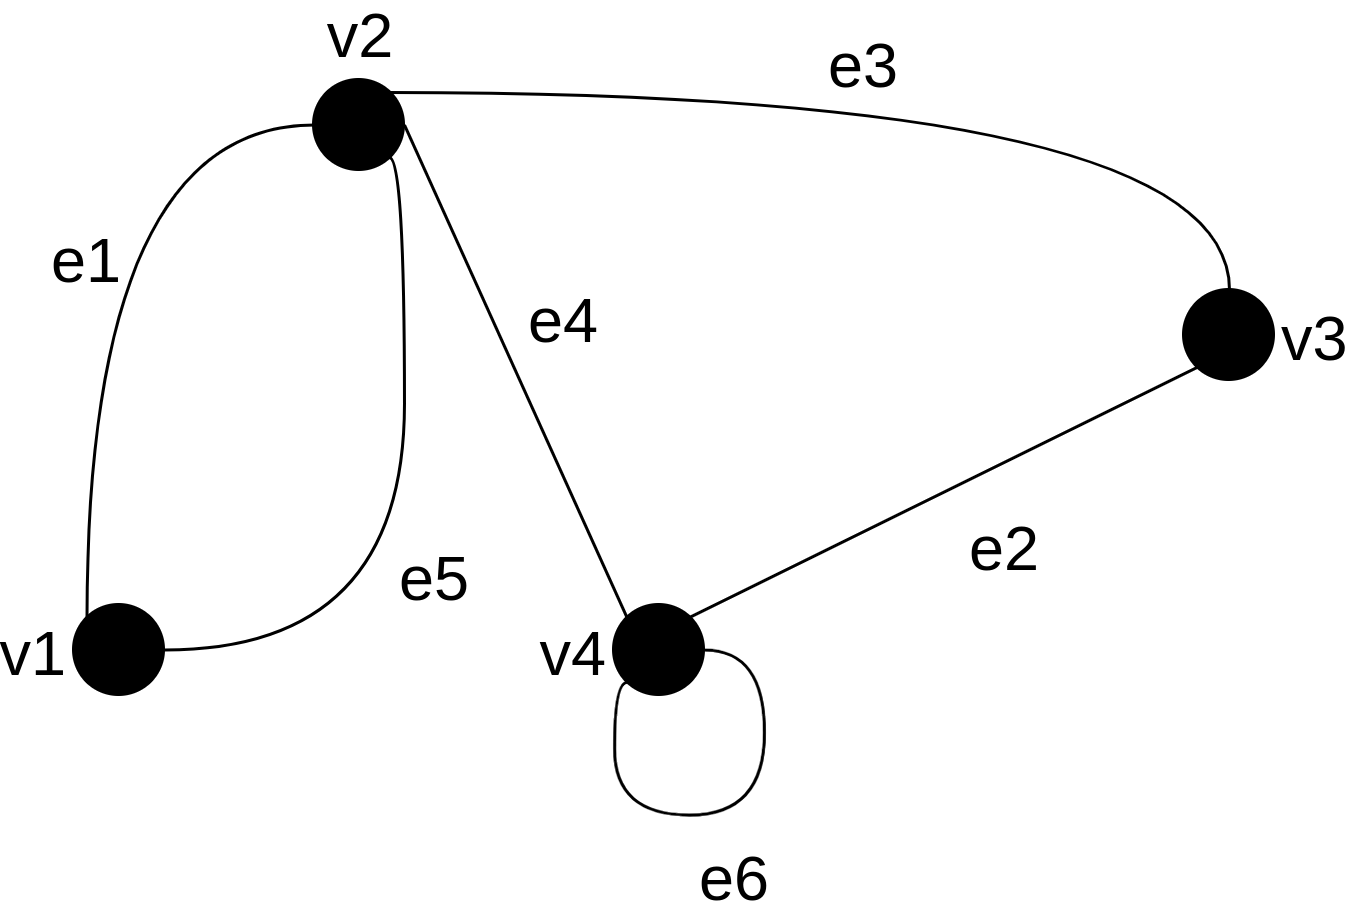
\includegraphics[width=0.8\textwidth]{images/graph_undirected.png}
    \end{center}
    \caption{Graphe non orienté}
    \label{graph_undirected}
\end{figure}
Un graphe orienté est semblable à un graphe non-orienté. La seule différence est qu'une direction 
est donnée au lien entre deux noeuds et ce lien ne se nomme plus "arête" mais "arc". La figure 
\ref{graph_directed} montre un exemple d'un tel graphe.
\begin{figure}
    \begin{center}
        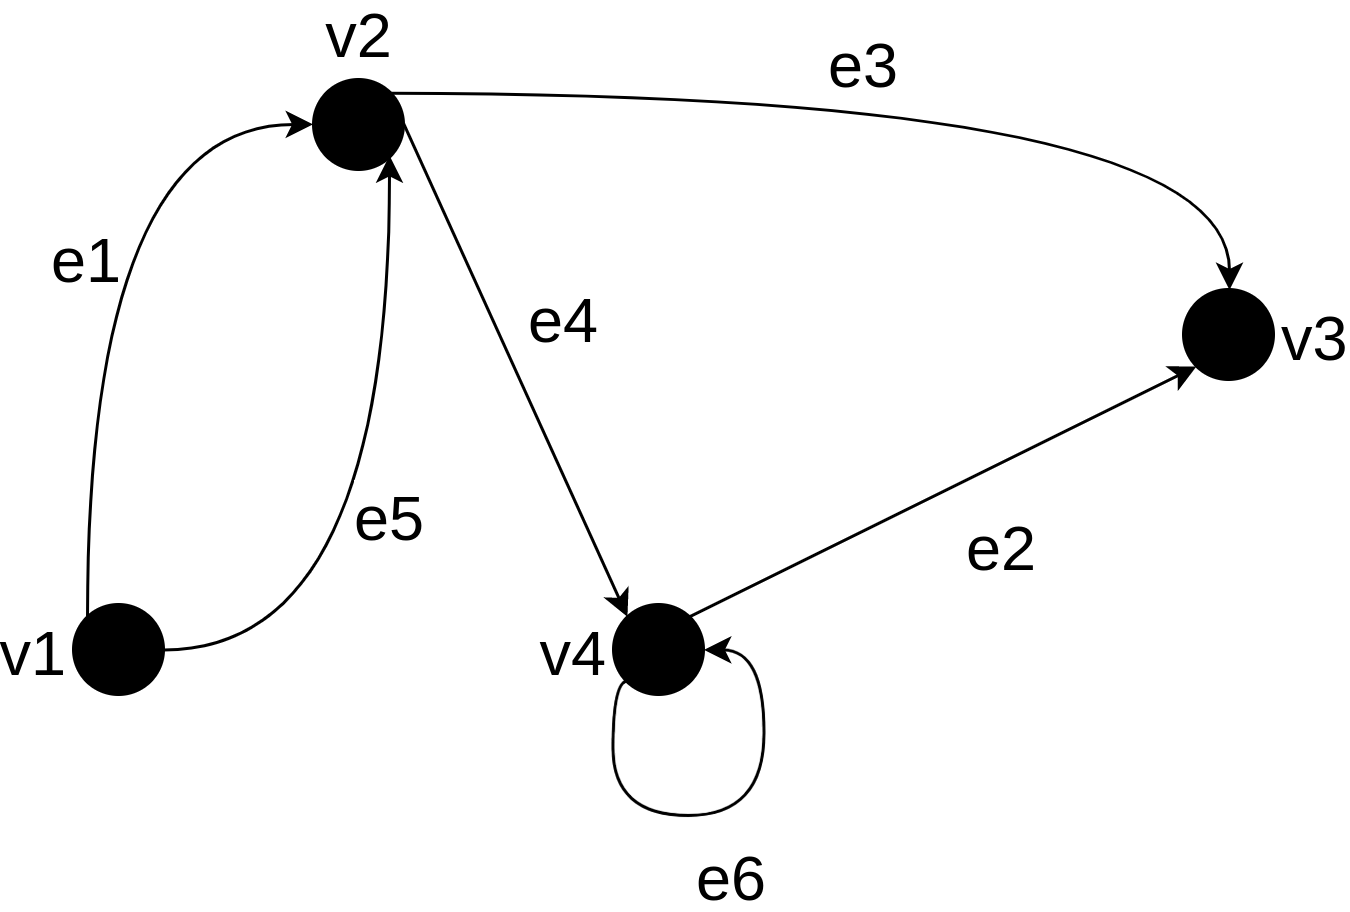
\includegraphics[width=0.8\textwidth]{images/graph_directed.png}
    \end{center}
    \caption{Graphe orienté}
    \label{graph_directed}
\end{figure}
Un graphe est donc un ensemble de noeuds reliés par des arêtes ou des arcs, selon si le graphe est 
orienté ou non. Dans notre cas, l'utilisation d'un graphe n'est pas si éloignée de celle d'un arbre. 
Par ailleurs, selon la théorie des graphes, "un arbre est un graphe sans cycle et connexe" (Hêche, 
page 33, \cite{ref28}). "Sans cycle" signifie qu'un parcours du graphe est possible de telle sorte 
à ce que le noeud de départ et d'arrivée soient différents. "Connexe" définit un graphe tel que 
pour chaque paire de noeuds du graphe il existe un chemin les reliant. L'utilisation d'un tel 
graphe représente fidèlement l'arborescence du \acrshort{fs} (on garde le schéma d'un arbre) 
et simplifie grandement les opérations lorsque des événements surviennent sur ce dernier. 
Le fait d'ajouter les tags comme noeuds du graphe 
maintient une unique structure de données cohérente et diminue le nombre d'opérations différentes 
nécessaires lors de la mise à jour du \acrshort{fs}. Le parcours de ce graphe se fait en 
fonction du chemin de fichier donné, en gardant l'identifiant unique du noeud correspondant au 
répertoire racine, le parcours se fait de la racine vers le noeud final du chemin de fichier.
\bigbreak
La table de hachage utilisée dans cette version peut être vue comme un "cache" d'accès aux noeuds 
tags. En effet, nous pourrions nous passer de cette table de hachage et lorsqu'un accès à un tag 
est demandé, rechercher dans tout le graphe le tag en question. Cependant, cette dernière opération 
devient rapidement conséquente lorsque le graphe comporte de très nombreux noeuds. De plus, cette 
\textit{hashmap} est accédée bien moins souvent que dans la première version de l'architecture, 
car elle est mise à jour uniquement lors des opérations sur les tags et non plus sur celles liées 
seulement aux fichiers et répertoires (opérations potentiellement plus lourdes).
\bigbreak
Comme pour la sous-section \ref{indexation_hashmap_arbre}, la table \ref{table_architecture_2} 
donne pour chaque événement survenu sur le \acrshort{fs}, les opérations 
à exécuter pour les deux structures de données (le graphe et la table de hachage) et une approximation 
de la complexité. Les événements sont représentés par leurs numéros, en table 
\ref{table_evenements_possibles}. Les variables suivantes sont définies :
\begin{itemize}
    \item c = Opération constante.
    \item p = Profondeur du graphe.
    \item t = Nombre de tags.
\end{itemize}
Nous pouvons constater que les opérations sur la table de hachage sont peu nombreuses et souvent 
facultatives, ce qui se traduit par un gain sur le nombre d'opérations totales.
\begin{center}
    \begin{tabularx}{16cm}{|c|X|p{5.5cm}|} \hline
        \textbf{Numéro} & \textbf{Opération graphe} & \textbf{Opération \textit{hashmap}} \\ \hline
        1 & Parcourir le graphe à la recherche du fichier, 
            si besoin créer le noeud tag, et relier le noeud fichier au noeud tag -> $O(p * c)$ 
            & Si non existant, ajouter le nom du tag comme clé et son identifiant dans le graphe 
            comme valeur -> $O(c)$ \\ \hline
        2 & Parcourir le graphe à la recherche du 
            noeud fichier et supprimer le lien entre noeud tag et fichier. Si le noeud tag 
            n'est relié à aucun autre noeud, le supprimer -> $O(p * c)$ & Si le noeud tag 
            n'est relié à aucun autre noeud, supprimer l'entrée -> $O(c)$ \\ \hline
        3 & Obtenir l'identifiant grâce à la hashmap et renommer le noeud correspondant -> $O(c)$ & 
            Supprimer l'entrée et en recréer une avec le nouveau nom et le même identifiant -> $O(c)$ \\ \hline
        4 & Parcourir le graphe à la recherche du répertoire parent, 
            ajouter le nouveau noeud. Pour les tags existants, lier le nouveau noeud, sinon créer 
            le nouveau noeud tag correspondant -> $O(p * t * c)$ & Pour chaque tag, opération identique 
            au numéro 1 \\ \hline
        5 & Parcourir le graphe à la recherche du répertoire parent, 
            ajouter le nouveau noeud. Pour les tags existants, lier le nouveau noeud, sinon créer 
            le nouveau noeud tag correspondant. Répéter pour la sous-arborescence -> $\approx 
            O(p^2 * t * c)$ & Pour chaque tag, opération identique au numéro 1 \\ \hline
        6 & Parcourir le graphe à la recherche du parent et 
            changer le lien du noeud avec son parent / simple renommage du nom dans 
            l'étiquette -> $O(p * c)$ & Pas d'opération requise \\ \hline
        7 & Identique au numéro 6 & Pas d'opération requise \\ \hline
        8 & Parcourir le graphe à la recherche du noeud fichier et supprimer les 
            liens entre noeuds tags et noeud parent -> $O(p * t * c)$ & Pour chaque tag du fichier, 
            supprimer le noeud tag s'il n'a plus de liens vers d'autres noeuds -> $O(t * c)$ \\ \hline
        9 & Parcourir le graphe à la recherche du noeud répertoire et supprimer les 
            liens entre noeuds tags et noeud parent. Répéter pour la sous-arborescence -> $\approx 
            O(p^2 * t * c)$ & Pour chaque sous répertoire ou sous fichier, opération identique au numéro 8 \\ \hline
    \end{tabularx}
    \captionof{table}{Opérations et complexité, deuxième architecture}
    \label{table_architecture_2}
\end{center}

%%%%%%%%%%%%%%%%%%%%%%%%%%%%%%%%%%%%%%%%%%%%%%%%%%%%%%%%%%%%%%%%%%%%%%%%%%%%%%%%%%%%%%%%%%%%%%%%%%%
%%%%%%%%%%%%%%%%%%%%%%%%%%%%%%%%%%%%%%%%%%%%%%%%%%%%%%%%%%%%%%%%%%%%%%%%%%%%%%%%%%%%%%%%%%%%%%%%%%%
\subsection{Surveillance du \acrshort{fs}}
La surveillance du \acrshort{fs} et des tags associés est le deuxième pilier du système. 
L'indexation initiale est nécessaire, mais il est également nécessaire de surveiller en permanence 
l'arborescence des fichiers pour garder cet index à jour. Pour y parvenir, nous allons utiliser 
\mintinline{c}{inotify} (voir section \ref{inotify_techno}), en surveillant tout particulièrement les événements 
suivants :
\begin{itemize}
    \item IN\_ATTRIB : changement sur les tags (ajout, suppression, renommage).
    \item IN\_CREATE : création de fichier/répertoire dans le répertoire surveillé. Ajouter une nouvelle surveillance si répertoire.
    \item IN\_DELETE : suppression d'un fichier/répertoire dans le répertoire surveillé.
    \item IN\_DELETE\_SELF : suppression du répertoire surveillé.
    \item IN\_MOVE\_SELF : suppression d'un fichier/répertoire dans le répertoire surveillé.
    \item IN\_MOVE\_FROM : déplacement/renommage du répertoire (ancien nom).
    \item IN\_MOVE\_TO : déplacement/renommage du répertoire (nouveau nom).
\end{itemize}
Un thread s'occupe d'écouter les événements du \acrshort{fs} et les inscrit dans un buffer 
tandis qu'un autre va mettre à jour le graphe pour répercuter les changements survenus en lisant 
dans ce même buffer (simple pattern producteur-consommateur).

%%%%%%%%%%%%%%%%%%%%%%%%%%%%%%%%%%%%%%%%%%%%%%%%%%%%%%%%%%%%%%%%%%%%%%%%%%%%%%%%%%%%%%%%%%%%%%%%%%%
%%%%%%%%%%%%%%%%%%%%%%%%%%%%%%%%%%%%%%%%%%%%%%%%%%%%%%%%%%%%%%%%%%%%%%%%%%%%%%%%%%%%%%%%%%%%%%%%%%%
\subsection{Requêtes de tags et fichiers}
Une fois que la surveillance du \acrshort{fs} est en place, le système doit pouvoir répondre 
à des requêtes de la part de l'utilisateur. À travers un outil en ligne de commande, l'utilisateur 
a la possibilité de : 
\begin{itemize}
    \item Demander la liste des fichiers et répertoires associés à un ou plusieurs tags. La requête 
        peut être sous la forme d'une expression logique simple (avec les opérateurs logiques "et" 
        et "ou").
    \item Demander la liste des tags déjà existants. 
    \item Renommer un tag. 
\end{itemize}
Pour échanger les requêtes et les réponses, client et serveur communiquent par sockets, avec un 
format de protocole très simple pour distinguer le type d'une requête.
